En este capítulo se aplicará lo expuesto en los capítulos 3 y 4 para realizar los experimentos correspondientes, y se describirán los resultados obtenidos.

\subsection{Introducción}
    
El último capítulo trata sobre el uso de los algoritmos y metaheurísticas aplicados sobre problemas reales de TSP, primero se explicará el proceso que se realizó y al final se mostrarán los resultados obtenidos.\\
\hspace*{1cm}Cada uno de los problemas de TSP se probará tanto con el método de cuadrantes como sin este método; en ambos casos se probará con algo conocido como "mutación" que alterará la solución base reordenando algunos de sus puntos con el fin de obtener resultados aleatorios pero coherentes. Como se muestra en la tabla \ref {table:DescripcionPruebasTSP} estos serán los problemas a utilizar obtenidos en la página de la Universidad de Heidelberg \cite {[TSPLIB]} y cuyas descripciones se obtuvieron de la Universidad de Waterloo \cite{[TSPLIB2]}.

% Please add the following required packages to your document preamble:
% \usepackage[table,xcdraw]{xcolor}
% If you use beamer only pass "xcolor=table" option, i.e. \documentclass[xcolor=table]{beamer}
\begin{table}[]
\centering
\caption{Descripción de los problemas de TSP usados para las pruebas.}
\resizebox{1\textwidth}{!}{
\rotatebox{0}{
\begin{tabular}{lcll}
\hline
\rowcolor[HTML]{9B9B9B} 
\multicolumn{1}{c}{\cellcolor[HTML]{9B9B9B}{\color[HTML]{FFFFFF} \textbf{Problema}}} & {\color[HTML]{FFFFFF} \textbf{Ciudades}} & \multicolumn{1}{c}{\cellcolor[HTML]{9B9B9B}{\color[HTML]{FFFFFF} \textbf{Descripción}}} & \multicolumn{1}{c}{\cellcolor[HTML]{9B9B9B}{\color[HTML]{FFFFFF} \textbf{Autor}}} 	\\ \hline
a280.tsp                                                                             & 280                                      & Problema de perforación						                                   		  & Ludwig                                   		  								  	\\ \hline
brd14051.tsp                                                                         & 14051                                    & Republica federal de Alemania en 1989                                                   & Bachem y Wottawa                                   		  							\\ \hline
ch150.tsp                                                                            & 150                                      & Problema de 150 ciudades							                                      & Churritz                                   		  									\\ \hline
d1655.tsp                                                                            & 1655                                     & Problema de perforación						                                          & Reinelt                                   		  									\\ \hline
d493.tsp                                                                             & 493                                      & Problema de perforación						                                          & Reinelt                                   		  									\\ \hline
eil101.tsp                                                                           & 101                                      & Problema de 101 ciudades 						                                          & Christofides y Eilon                                   		  						\\ \hline
fl417.tsp                                                                            & 417                                      & Problema de perforación 					                                           	  & Reinelt                                   		  									\\ \hline
lin318.tsp                                                                           & 318                                      & Problema de 318 ciudades				                                                  & Lin y Kernighan                                   		  							\\ \hline
p654.tsp                                                                             & 654                                      & Problema de perforación					                                              & Reinelt                                   		  									\\ \hline
pcb3038.tsp                                                                          & 3038                                     & Problema de perforación 								                                  & Reinelt y Juenger                                   		  						\\ \hline
rd400.tsp                                                                            & 400                                      & Problema de aleatorio de 400 ciudades			                                          & Reinelt                                   		  									\\ \hline
rl5934.tsp                                                                           & 5934                                     & Problema de 5934 ciudades				                                                  & Reinelt                                   		  									\\ \hline
u159.tsp                                                                             & 159                                      & Problema de perforación						                                          & Reinelt                                   		  									\\ \hline
u724.tsp                                                                             & 724                                      & Problema de perforación						                                          & Reinelt                                   		  									\\ \hline
vm1084.tsp                                                                           & 1084                                     & Problema de 1084 ciudades			                                                      & Reinelt                                   		  									\\ \hline
\end{tabular}
}
}
\label{table:DescripcionPruebasTSP}
\end{table}



%Gerhard Reinelt
%Ludwig
%Bachem
%Wottawa
%Churritz
%Christofides
%Eilon
%Lin
%Kernighan
%Juenger 

\subsection{Procedimiento}
\subsubsection{Mutación de la solución base}
Una mutación consiste en obtener un resultado distinto en base a uno fijo, para ello se usará el concepto de Especie, una especie es un conjunto de variables numéricas compuestas por 2 arreglos del mismo tamaño, estos arreglos se llaman respectivamente cromosomas y genes cuya función se explicará a continuación.\\
\hspace*{1cm}Como se explicó con el método de cuadrantes, la constante división en partes más pequeñas permite realizar cálculos más rápidos; al momento de trazar una ruta se espera que el siguiente destino sea el más cercano al lugar de donde se partió y el uso de cuadrantes permite crear zonas aisladas donde algunos de los puntos se encuentran más cerca entre sí.\\
\hspace*{1cm}Sin embargo, ¿qué pasa si hay un punto más cercano a un grupo, pero debido a la división hecha por el algoritmo se ubica en un cuadrante diferente? En este caso se perdería un importante ahorro de distancia.\\
\hspace*{1cm}Para solucionar este problema se hará uso de las metaheurísticas creando especies de valores aleatorios permitiendo alterar la solución base y así obtener una solución diferente.\\
\hspace*{1cm}Como ejemplo se mostrará el problema eil51.tsp; en la figura \ref {fig:eil51_original.png} se muestra la solución obtenida por el método de cuadrantes con el resultado de 507 unidades de distancia, sin embargo se puede mejorar como muestra el recuadro dentro de la figura mencionada.

     \begin{figure}[hbtp]
        \centering
            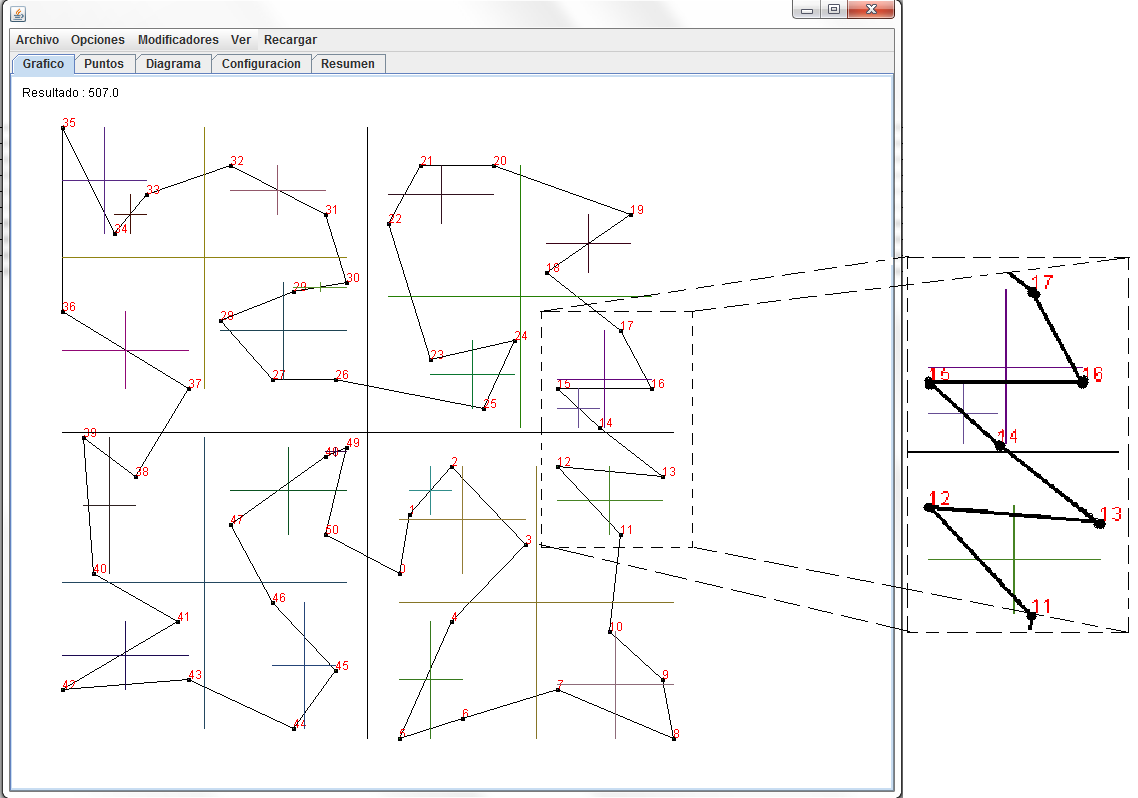
\includegraphics[width=0.7\textwidth]{PruebasResultados/Imagenes/eil51_original_recuadro.png}
            \caption{Problema eil51.tsp resuelto por el método de cuadrantes.}
            \label{fig:eil51_original.png}
    \end{figure}
    
\hspace*{1cm}Como se ha mencionado anteriormente, una especie está formada por 2 arreglos, cada arreglo tiene uno de estos valores: el gen que se encargará de seleccionar uno de los puntos y el cromosoma que indicará hacia donde se desplazará el intercambio; el objetivo de la especie es reordenar los puntos seleccionados, y debido a que ya se resolvió el problema con el método de cuadrantes, no es necesario hacer intercambio con todos los elementos de la lista sino solo con los más cercanos.\\

\hspace*{1cm} En la figura \ref {fig:eil51_explicado.png} se podrá ver que se generó una especie formada por 2 arreglos, una señala al punto 11 y otro al 12,en ambos indica como tipo de cromosoma el número 2. El proceso se dividió en 3 fases:
 \begin{figure}[hbtp]
        \centering
            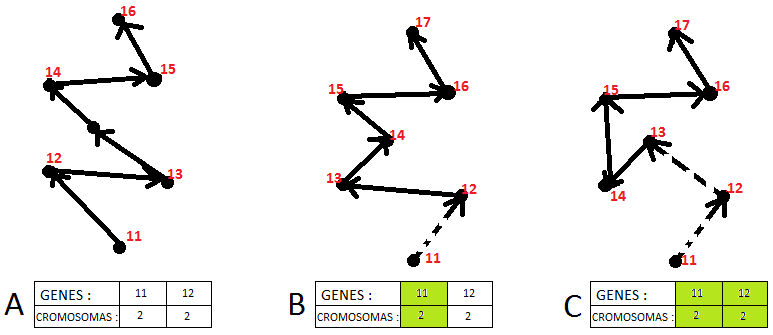
\includegraphics[width=0.75\textwidth]{PruebasResultados/Imagenes/eil51_explicado.png}
            \caption{Problema eil51.tsp resuelto por el método de cuadrantes con una especie aplicada.}
            \label{fig:eil51_explicado.png}
    \end{figure}
\begin{itemize}
    \item \textbf{A:} Éste es el tramo inicial que donde se puede observar que aún no se ha modificado el segmento de la ruta.
    \item \textbf{B:} Aquí se hace el reemplazo, el gen marca el punto 11 y el cromosoma 2, eso quiere decir que el punto 11 tendrá  como siguiente objetivo aquél que este 2 lugares delante de él (13), se intercambiarán las posiciones 12 con el 13, generando una nueva ruta, a diferencia de la fase A, el punto 12 y 13 se encuentran en lugares distintos.
    \item \textbf{C:} Por último se repite lo mostrado en la fase B, esta vez con el nuevo punto 12 y el 14, de nuevo intercambiarán posiciones los puntos 13 y 14 volviendo a generar una nueva ruta.
\end{itemize}

\hspace*{1cm}En la figura \ref {fig:eil51_recocido.png} se muestra la ruta completa con el cambio realizado que tendrá de resultado 502 unidades de distancia, ahorrándose 5 unidades. Este ejemplo es solo hipotético, y para que pueda funcionar se tendrán que hacer varias generaciones de especies, algunos haciendo movimientos para llegar a dicha solución, además de que el reordenamiento puede generar rutas más cortas pero a su vez otras más largas. El objetivo de este procedimiento es ir refinando las especies generadas con el fin de obtener una que mejore la solución obtenida.
     \begin{figure}[hbtp]
        \centering
            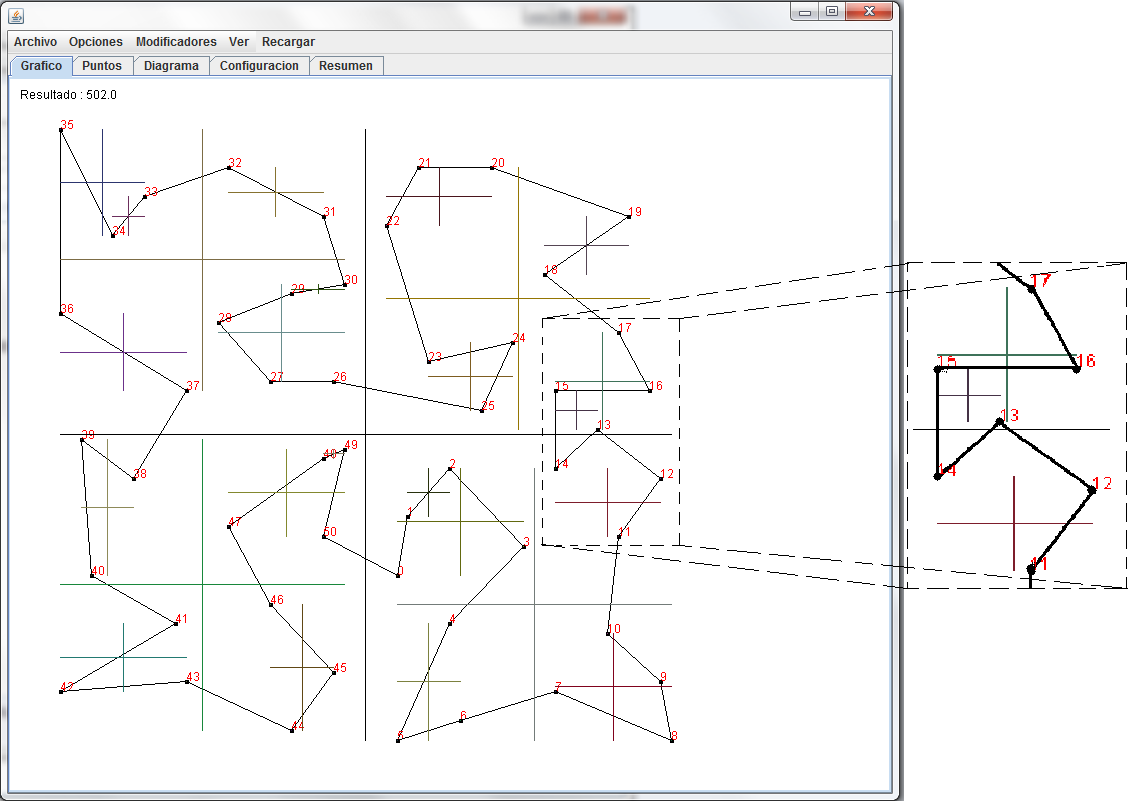
\includegraphics[width=0.7\textwidth]{PruebasResultados/Imagenes/eil51_recocido_recuadro.png}
            \caption{Problema eil51.tsp resuelto por el método de cuadrantes explicando cómo funciona el uso de las especies.}
            \label{fig:eil51_recocido.png}
    \end{figure}    